This year saw great progress for the Open Data Lab. Early on there were weekly meetings to define goals and objectives. Those meetings lead to implementation of several areas and this chapter presents the key developments during 2018.

\section{Phase 1 Closed Beta}
The first decision made for the Open Data Lab was to implement a staged approach. Section~\ref{phases} summarizes the whole scope. This section discusses the state of the closed beta (Phase 1). The user base for this phase is predominantly the Data Science Institute. There were 116 participants ranging from students, to faculty, to staff. There were also 26 workshop attendees ranging from a diverse selection of UVA researchers to community members.
The primary goal of this phase is to test different technology solutions to anticipated needs (see section~\ref{techsolu}). Those range from data storage to computation to discovery to pedagogy, and so on. Of particular note was the wild success of implementing Project Jupyter. The tools developed by this project served many roles (see section~\ref{sec:projectjupyter}).
This phase will run until several criteria are met. The first is the establishment of a new funding model that will cover the scope of the open beta test. The second is the acquisition of new staff. Currently the Open Data Lab has a bus factor of one and phase 2 requires a higher value. 

\section{Establishment of User Base}
This year saw the birth of the Open Data Lab and growth to include 116 users. Those users take various form from capstone research programs at the graduate and undergraduate level to full fleged dissertation research. Some of the users involved are dealing with datasets that now reside within the Open Data Lab. Currently those datasets and under tight restriction as we explore proper security protocols. There is also a contingent of undergrad and graduate students that are part of data science clubs at UVA who gain access to resources through the Open Data Lab.

It is important to understand that the technology behind the system is not the driver of the system. The needs of the user are the driver. Right now the closed beta format allows us to interview new users and tailor a program to them. Sometimes we get the resource wrong and adjustments have to be made.
Regarding data storage the use of S3 storage from Amazon Web Services has served a broad selection of users well. Recent developments in AWS object storage technology enable users to use it as if it were block storage. As a result S3 has proved an effective solution both for large scale data storage as well as database query repositories.
Providing computational resources has been guided by the user base as well. As the base grew it became clear that the notebook technology developed by Project Jupyter was highly effective and actually resulted in more people volunteering for the closed beta test. The use of that technology helped bring users into the system.


\section{Technology Exploration}
\label{techsolu}
Many different technologies were tested in 2018. Many options using Amazon Web Services were explored and those services were found to be excellent. Local UVA resources were also used and in particular the UVA HPC portal developed out of the VP-IT's office is phenomenal. Collaboration is also underway with the UVA library regarding the discovery component of the Open Data Lab and the implementation of Harvard's Dataverse, known locally at UVA as Libra. For version control and sharing purposes GitHub was evaluated.

\subsection{Amazon Web Services}
Cloud computing provides agility that local computational resources do not. To that end we established a contract with Amazon Web Services (AWS) through the third-party vendor DLT solutions. This contract is collectively negotiated and takes advantage of the Internet-2 network \cite{ref:i2}.

In selecting a cloud resource provider our choice was informed by the needs of the  MSDS students at the DSI. The most requested cloud service was AWS and the plurality of job postings that are interested in cloud skills prefer AWS. During 2018 the initial scope of the AWS exploration was for functionality on colocating data and computation. However the initial implementation was more sucessful than anticipated. The system was popular and as a result Pete Alonzi functionally become the sysadmin for the DSI AWS account. What started as a development project turned into an operations project as soon as a minimum viable product was established. This is great for the DSI because there is a now a new resource for the researchers. However it did pull substantial resources from the development of the Open Data Lab.

In the following sections we will breakdown the different services used by the ODL.

\begin{table}[htbp]
\begin{center}
\begin{tabular}{lccr}
\hline
\hline
Service & Function & Notes \\
\hline
\hline
S3 & Object Storage & \$30/TB/yr \\
EC2 & Compute Instances & \href{https://aws.amazon.com/ec2/pricing/on-demand/}{pricing} \\
SageMaker & Project Jupyter & popular interface \\
IAM &  Identity/Access Manager  & users and groups \\
API Gateway & Credentialed REST & allows trigger of lambda \\
Lambda & Serverless Functions & miscellaneous tasks\\
CloudWatch & Log/Monitor/Alarm &  system monitor\\
\hline
\hline
\end{tabular}
\caption[AWS evaluation summary]{Summary of Amazon Web Services evaluated in 2018}
\end{center}
\end{table}

\subsubsection{S3}
This service provides the cheapest usable storage solution at scale. Furthermore recent policy developments at Amazon now require that other services interact with S3 (object storage) with comparable performace to block storage. That policy aligns nicely with the ODL needs. It means that cheaper Object Storage can be used for larger and larger datasets without yielding performance. Additionally this means only one storage solution needs to be implemented. We do not need to provision additional block storage for execution operations requiring data migration.

The S3 systems divides the data into buckets. For this test we treated a bucket as the unit holding data for a particular research project. As a result we have 22 buckets provisioned to accomodate all of our efforts. All buckets on AWS are localized to a region but must have a globally unique name. To that end for phase 1 we have adopted the following convention. Each bucket id begins with 'odl-' and is followed by the four character project id (eg: odl-hmtt).

\begin{table}[htbp]
\begin{center}
\begin{tabular}{lccr}
\hline
\hline
ID & Project \\
\hline
\hline
odl-bamc & Bourne/Mura Capstone  \\
odl-bamc-scratch & Bourne/Mura Capstone  \\
%odl-cbwc &  \\
odl-dome & Dominion Capstone \\
odl-hmtt & Healthy Markets \\
odl-hmtt-scratch & Healthy Markets  \\
odl-nept & Numismatic Linked Open Data  \\
odl-orci & Educational Open Datasets  \\
%odl-pmis &  \\
odl-podc & DSI Communications  \\
odl-projhects-test & DSI project configurations  \\
odl-readonly-test & read only test  \\
odl-scratch-test & scratch space test  \\
odl-sp19-sys6016 & Class materials  \\
odl-spark-education & Spark Educational Materials  \\
odl-spark19spds6003-001 & Class Materials  \\
odl-watr & Women and Terrorism Recruitment  \\
odl-watr-scratch & Women and Terrorism Recruitment  \\
odl-wiki & Wiki Capstone  \\
\hline
2017-2018-capstone-plos & 17/18 capstone  \\
uva-bucket & initial test bucket  \\
%846033058400-dlt-utilization & DLT bucket & part of DLT contract \\
\hline
\hline
\end{tabular}
\caption[S3 bucket summary]{Summary of S3 Buckets Provisioned for ODL 2018}
\end{center}
\end{table}

For the example of 'odl-hmtt' this bucket serves the Healthy Markets project. We bill that project PTAO for the service the ODL provides. The mechanism is to pay the DLT contract off the ODL PTAO and then do a cost transfer annually from the Healthy Markets PTAO to the ODL PTAO.

\subsubsection{13\,TB Data Transfer}
When we acquired the Healthy Markets dataset we transferred it from their aws bucket to ours. However this transfer was not trivial. AWS was unwilling to change the bucket ownership from their account to ours necessitating a data transfer.

The recommendation was to use the AWS CLI to perform the copy. It functions very similarly to scp from standtard unix systems. However we discovered several interesting features.
\begin{itemize}
\item Some of the files were copied to our bucket using an IAM account on their AWS account. Then Healthy Markets deleted that IAM user and as a result we lost control of the files in our bucket. We had to ask our partner to reestablish the account and then update the ownership. To do that we copied the files onto themselves but using our account so they would be owned by us. You cannot change the owner of a file on S3.

\item Direct bucket to bucket transfer is managed via a serverless operation and does not prototype the transfer. As a result the resources allocated automatically were not sufficient to transfer 13\,TB during a human lifetime. We then setup a dedicated server via EC2 and were able to configure the system to complete the transfer at a rate of about 4\,TB per day. We did incur cost for operating that server but is was not prohibitive.
\item The AWS CLI is not optimized for mass transfer and to copy the data in a reasonable timescale we had to write some scripts to chunk the operation. That work is located on the \href{https://github.com/UVA-DSI/Open-Data-Lab/tree/master/aws/large_s3_transfer}{ODL github page}.
\end{itemize}

\subsubsection{EC2}
This service allows for provisioning of compute resources. We established lambda functions to automate the create of EC2 instances for projects given a json configurationf file. Here is a sample JSON file:

\begin{verbatim}
{
   "projectId": "open-data-lab",
   "github": "https://github.com/UVA-DSI/Open-Data-Lab.git",
   "data-bucket": "odl-hmtt",
   "scratch-bucket": "odl-scratch-test",
   "ImageId": "ami-b70554c8",
   "InstanceType": "t2.nano",
   "email": "lpa2a@virginia.edu",
   "maxNumInstances": "1"
}
\end{verbatim}

These EC2 units are monitored by the CloudWatch system and we can configure them to turn on and off as necessary. The majority of our users use EC2 as their compute engine however they access the compute via auto-provisioning from the SageMaker service.


\subsubsection{SageMaker (Project Jupyter)}
\label{sec:projectjupyter}

SageMaker has been the breakout star of the 2018 ODL development phase. Our MSDS students prefer Project Jupyter as their mechanism for using computational and storage resources. To that end Peter Alonzi went to the JupyterCon in New York City in the fall of 2018\footnote{\url{https://github.com/UVA-DSI/conferences/tree/master/JupyterCon18}}.
At this conference Peter Alonzi was able to speak directly with the creators, developers, and users of Project Jupyter as well as the AWS developers of SageMaker. This service through the power of Project Jupyter is able to democratize the access and management of computational resources. The systems lifts a large cognative load off the user and empowers them to accomplish their goals efficiently without requiring arcane knowledge of computers. Our working metaphor is as follows:

\begin{quote}
\textbf{
The user is able to drive the car and get where they want to go without needing to first learn how to build a transmission.
}
\end{quote}

This power is the true killer feature of Project Jupyter and is the reason the system is so popular and widely used. Often people we say the ability to break code into cells and use markdown and inline plotting is the killer feature but it is really the lifting of the cognitive load.

\subsubsection{IAM}
This services governs Identity and Access Management. It breaks down into users and groups. Users are placed into appropriate logical groups and then access policies are assigned to groups.
When testing permission settings a dummy IAM user is established and given the same groups as the user being tested. In that way the sysadmin can see what the user sees and debug/test/prepare the system to the user.
\subsubsection{API Gateway}
We configured an API gateway to provide a mechanism for the users to trigger lambda functions. The users require credentialing via the standard aws authentication protocol when the post to the Gateway. \href{https://github.com/UVA-DSI/Open-Data-Lab/blob/master/aws/api-gateway/hitapi.py} Details of the system are on GitHub\footnote{\url{https://github.com/UVA-DSI/Open-Data-Lab/blob/master/aws/api-gateway/hitapi.py}}.
%\begin{verbatim}
%requests.post('https://pish6mpnr0.execute-api.us-east-1.amazonaws.com/alpha-2/%vm_stand_up',
%                        auth=auth,
%                        params={'projectID':sys.argv[1]})
%\end{verbatim}



\subsubsection{lambda}
This services allows for serverless execution of code. Currently we use it for provisioning of EC2 instances and automation of EC2 management.


\subsubsection{CloudWatch}
This service is how we monitor the system and record logs.

\pagebreak
\subsubsection{Architecture Diagrams}


\begin{figure}[!hbtp]
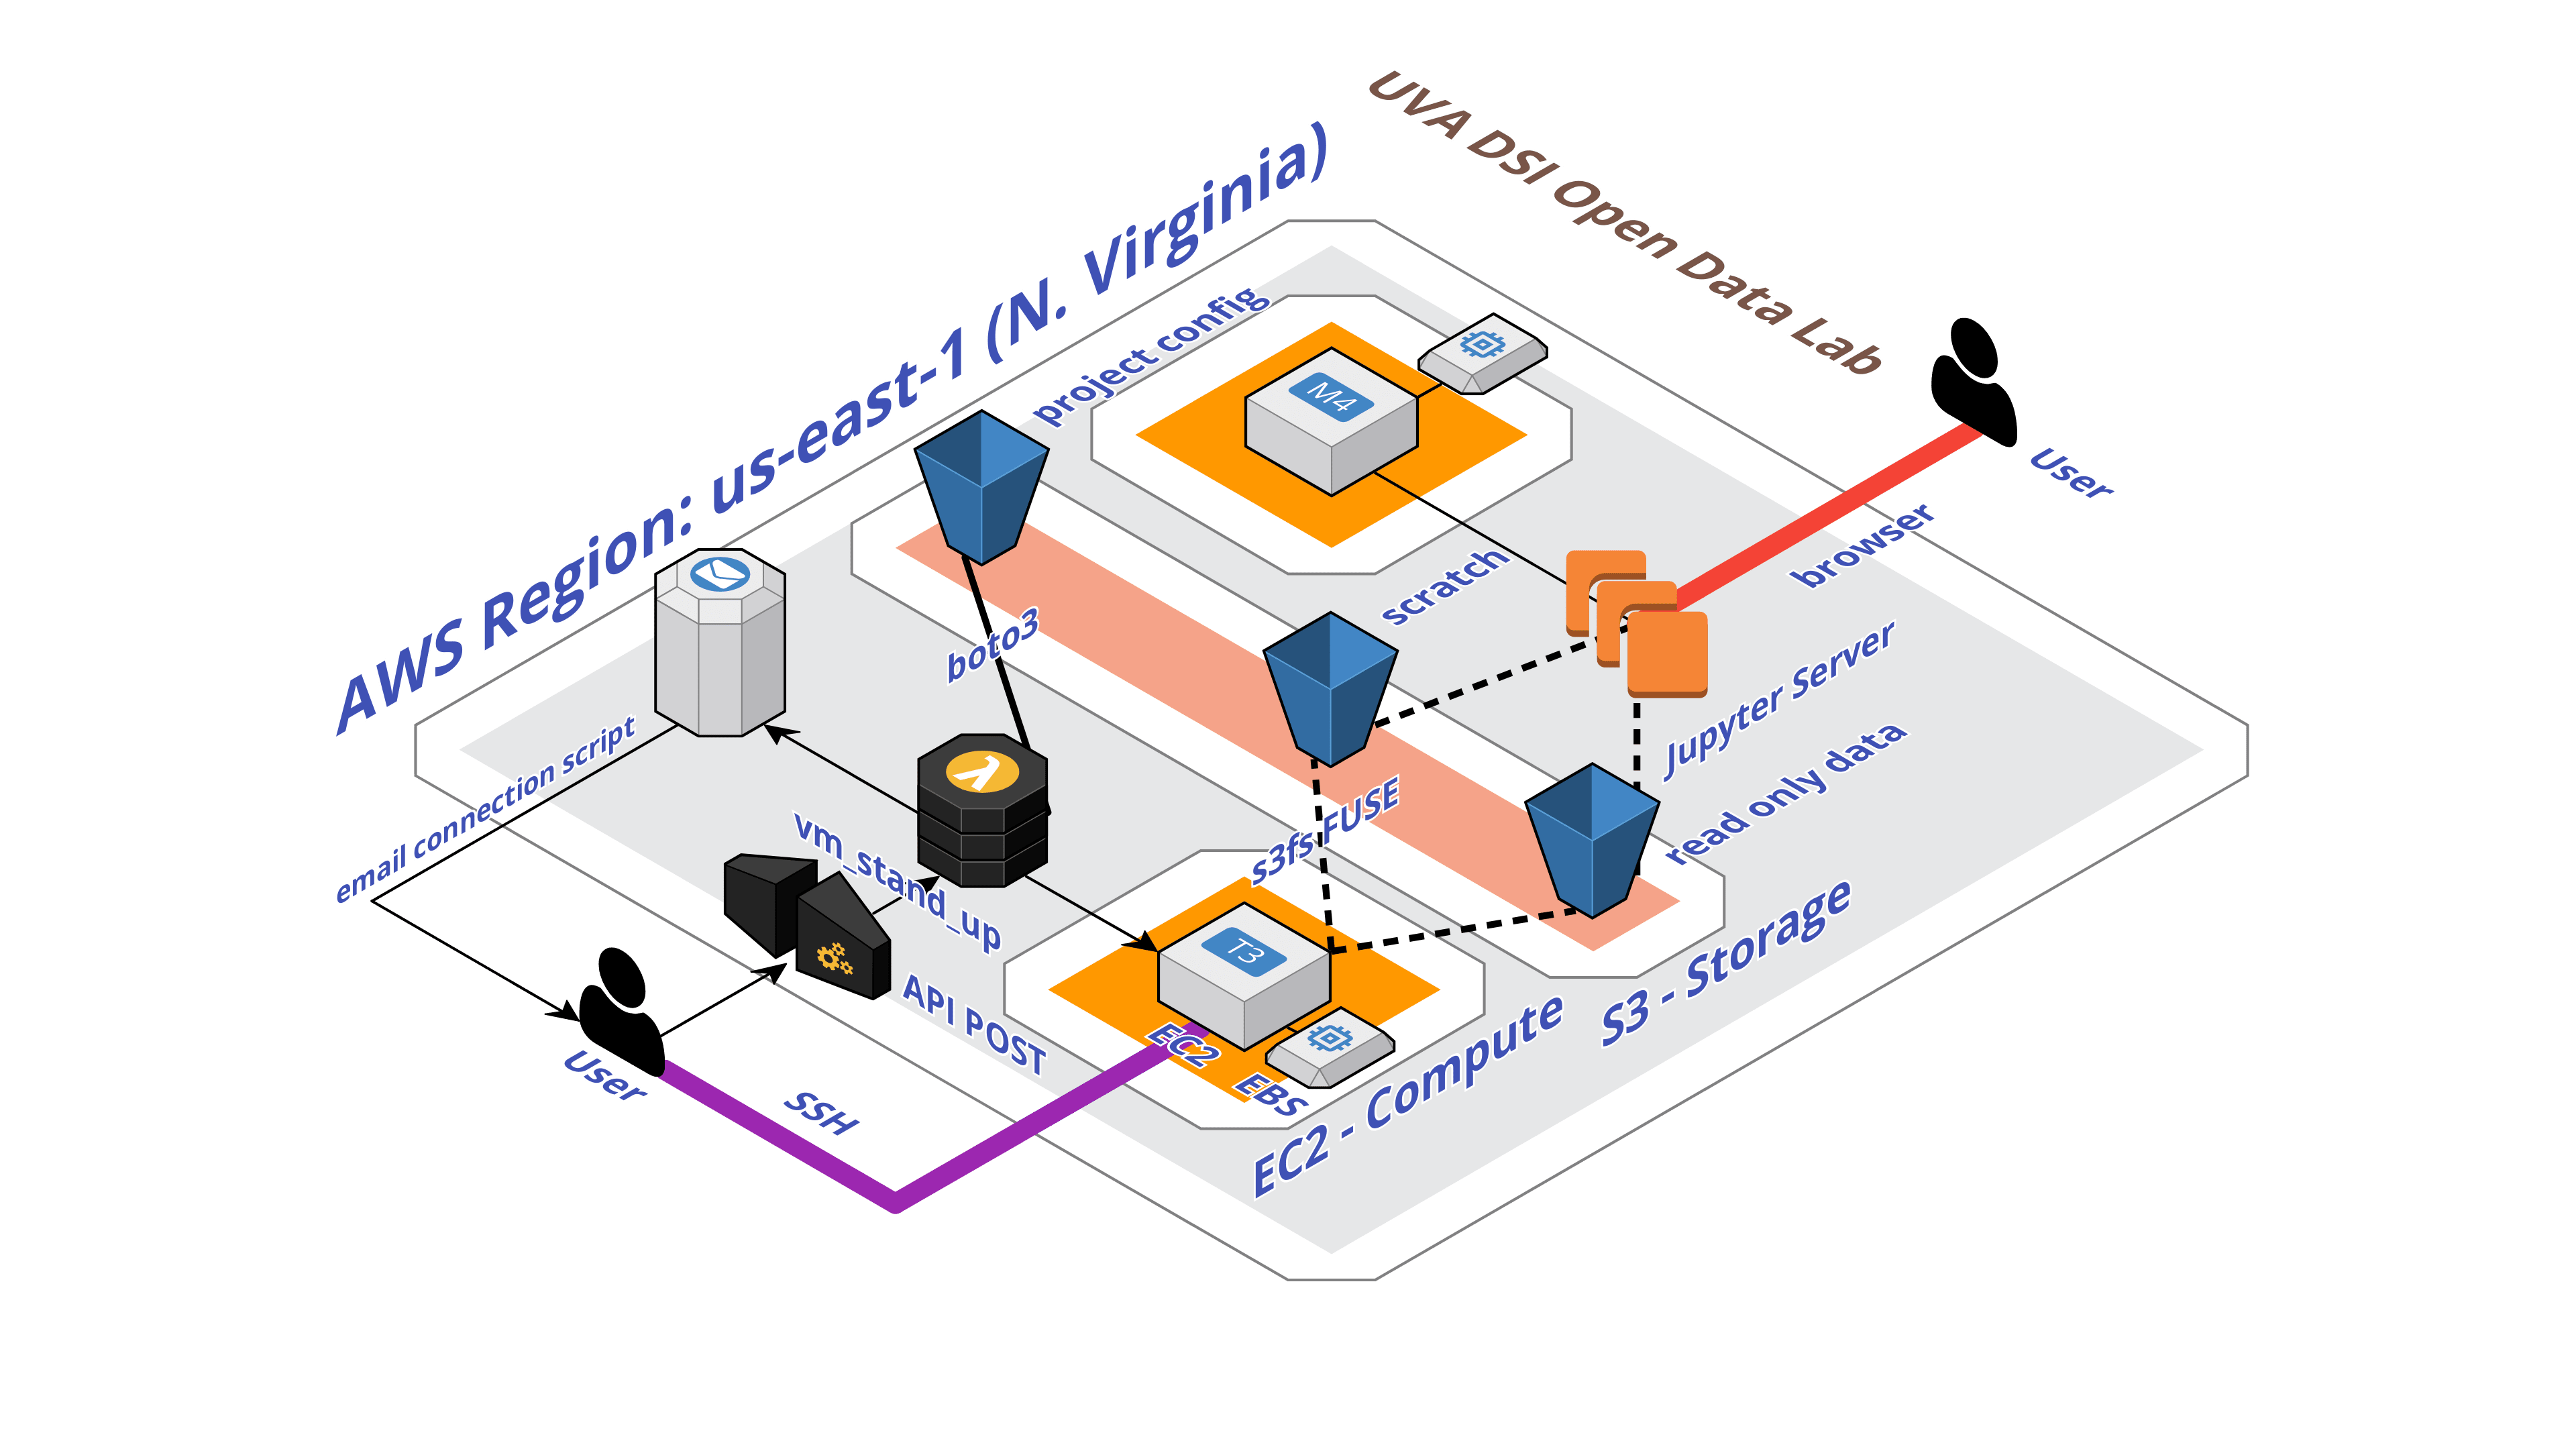
\includegraphics[width=0.97\textwidth]{images/odl-diagram.png}
\caption{Schematic of AWS service configuration\label{fg:aws}}
\end{figure}
\begin{figure}[!hbtp]
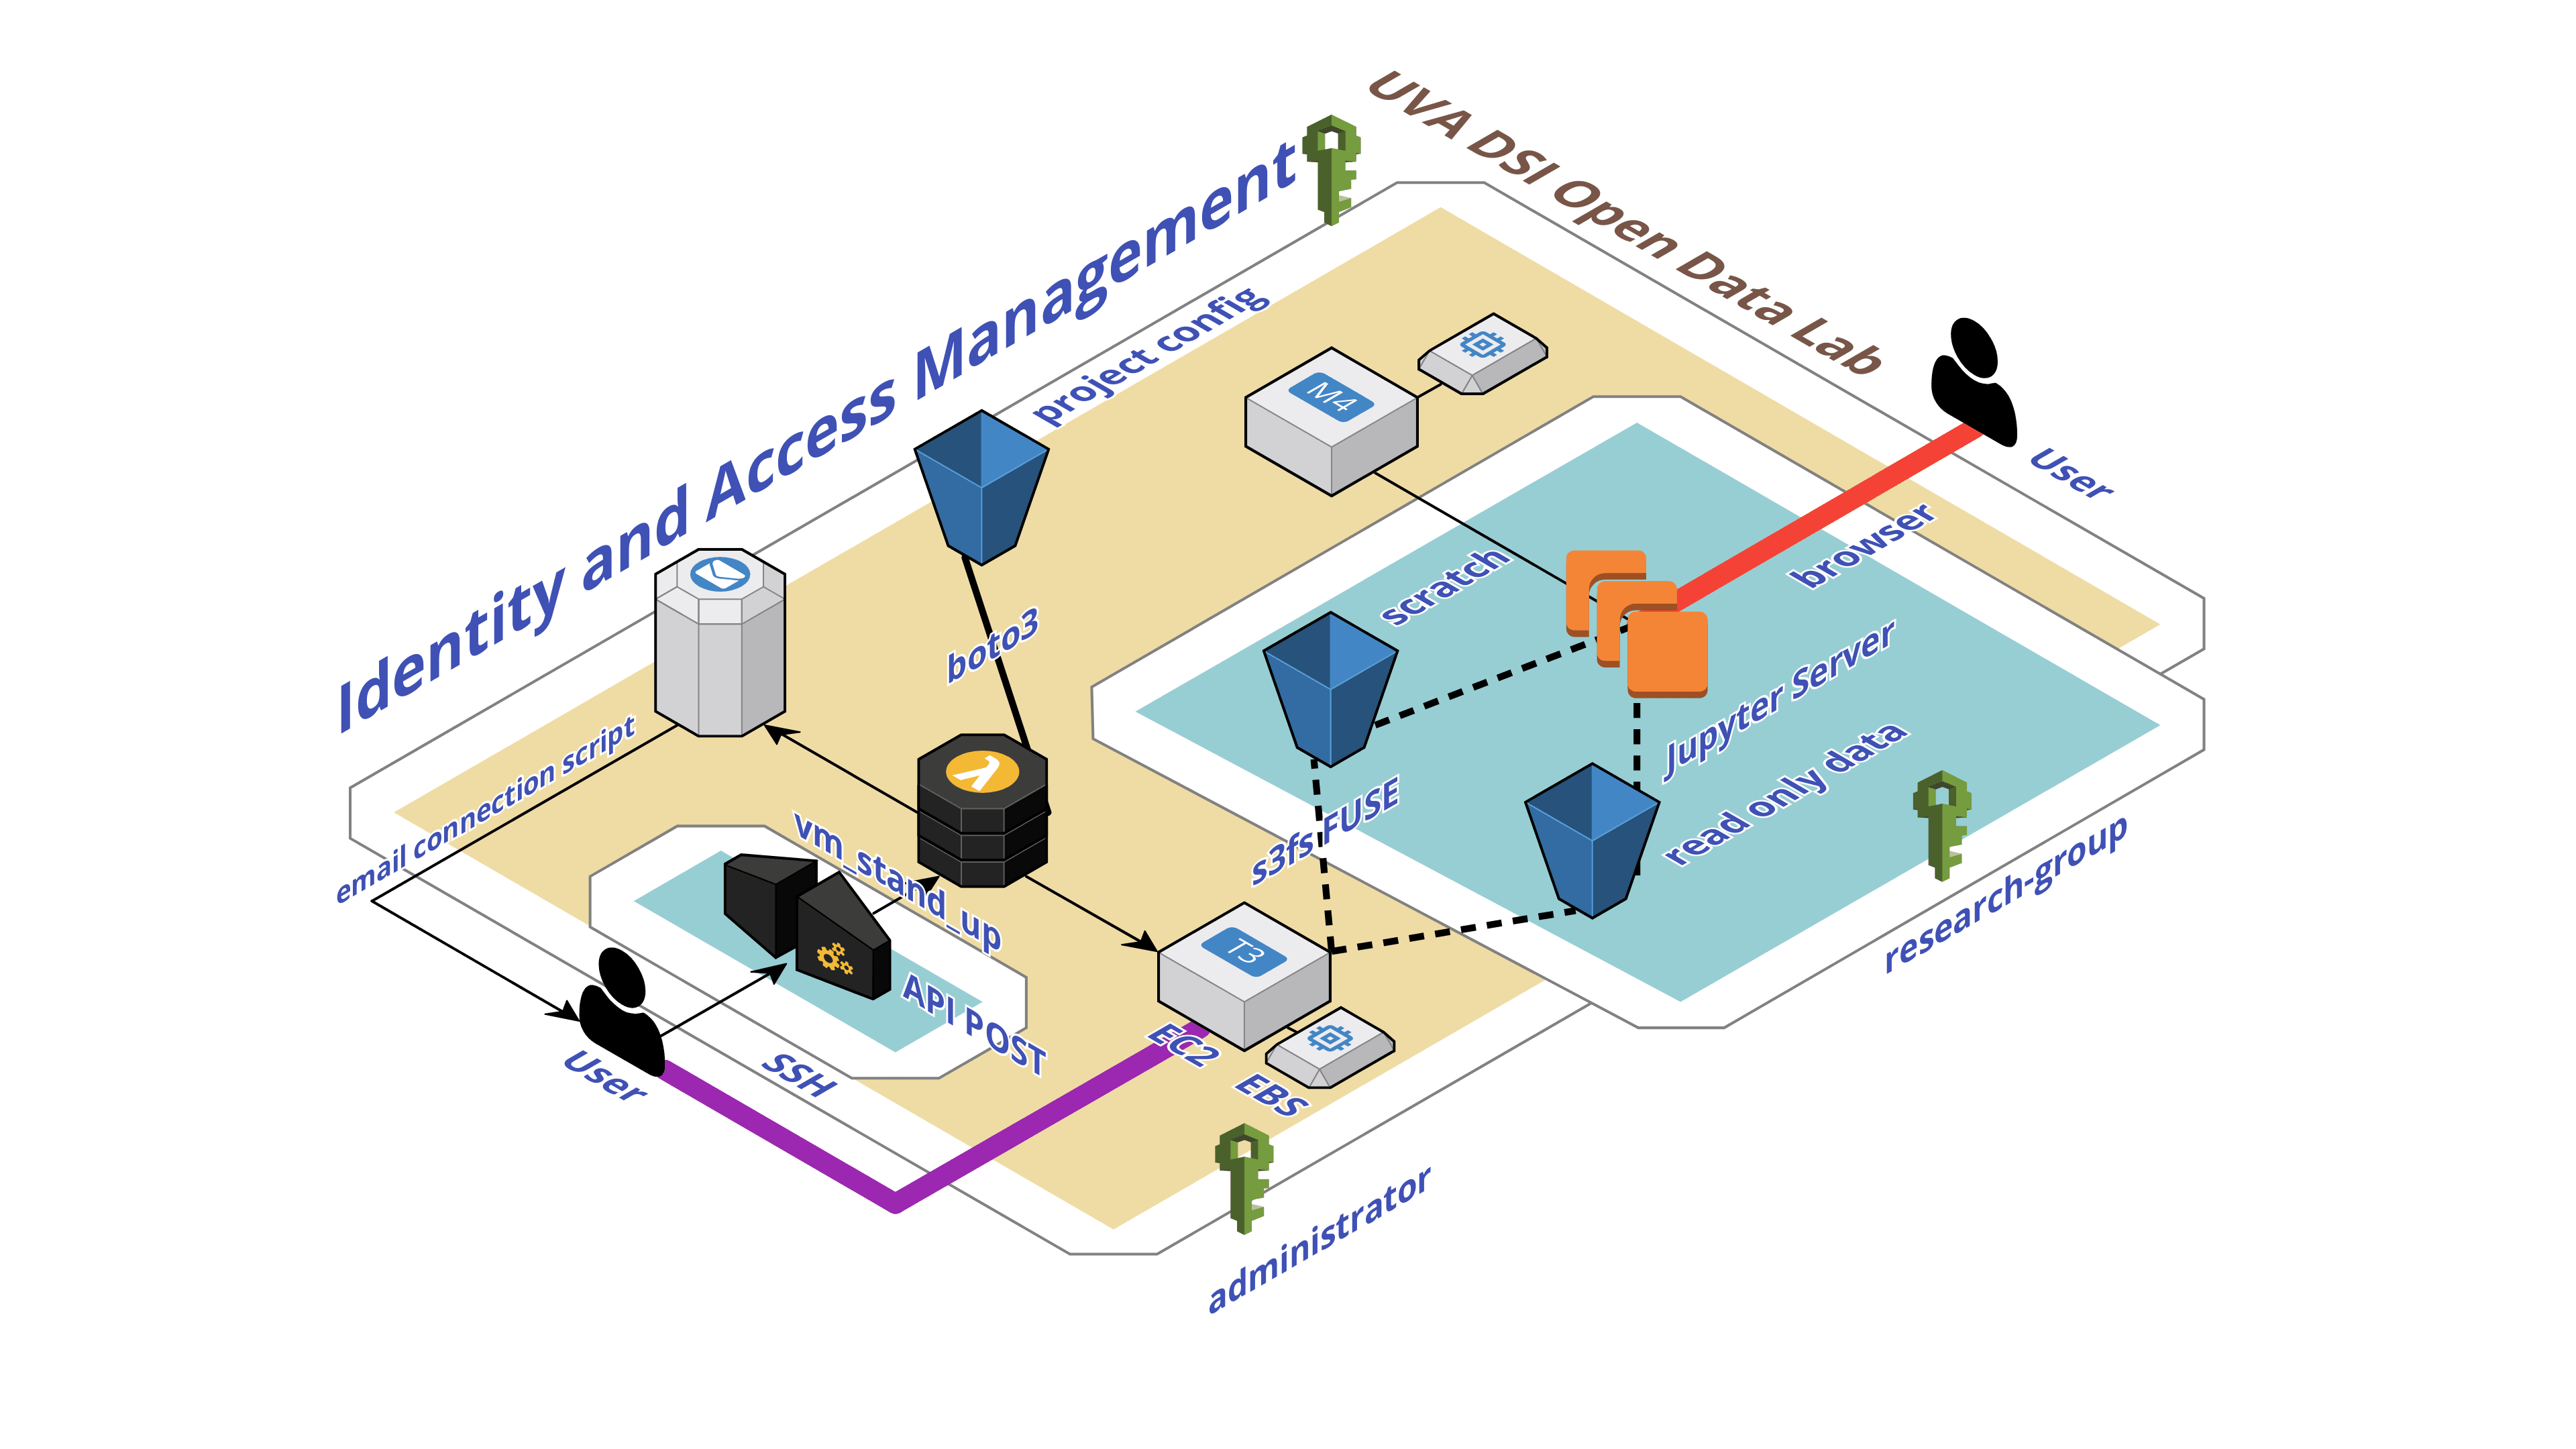
\includegraphics[width=0.97\textwidth]{images/odl-iam.png}
\caption{Schematic of AWS IAM configuration\label{fg:iam}}
\end{figure}



\subsubsection{Support Plan}
For the first year of the ODL we elected to keep the business support plan. In the future we can have a ten percent savings by eliminating this support.
\begin{verbatim}
https://aws.amazon.com/premiumsupport/compare-plans/
\end{verbatim}

\subsection{Local UVA - Rivanna and Ivy}
The local computational resources at UVA are facilitated through the office of Vice President for IT. That group is dedicated and hard working and provides great resources to the local UVA community. We have established a working relationship with them and discuss technical problems and solutions. Independently we arrived at the utility of Project Jupyter.
These solutions are for UVA personnel and their collaborators and as such will not scale to later phases of the Open Data Lab project. However for the closed and open beta it is a great resource. Furthermore their technical expertise will be invaluable to the Open Data Lab regardless of phase.

\subsection{GitHub}
GitHub is the most broadly adopted cloud platform for version control. Therefore we evaluated it first. The utility for managing repositories is fully mature. The collaborative features focused around the fork and pull request paradigm are excellent. GitHub also has project level capability with issue tracking and team/permission functionality for managing permissions and progress. We have been extremely pleased with the capabilities of GitHub. The only motivation to try other solutions is for the sake of due diligence.

Concerning the acquisition by Microsoft: Many have raised the issue that GitHub may not be the appropriate solution now that Microsoft has acquired GitHub. However the recent track record of Microsoft is to not meddle with projects like GitHub but rather to protect them. Additionally most users use other Microsoft products. 

We developed a workflow for beginning users on the GitHub platform. Details are given in~\ref{sec:git}.

\section{Upcoming Technical Exploration}
The following sections describe exploratory work that is on the schedule. There is more to be done beyond this list but not scheduled.
\subsection{Dataverse}
A framework has been outlined to use Dataverse as the discovery mechanism for the Open Data Lab. In this system a metadata entry will be made in the Dataverse containing all of the usual materials. However the final piece with the datafiles will contain pointers to the data and projects within the Open Data Lab. Dataverse is not configured for colocating computation resources with the data resources. The pilot of this test will be with the Libra project from the UVA Library. Currently that system is undergoing an upgrade and once there is a stable release exploration will commence.
\subsection{Spark}
The first scale data solution the Open Data Lab will explore is Spark. Preliminary work so far as been the development of a introductory workshop on the technology (available on the Open Data Lab github repository). A second pedagogical series will be presented early in 2019 and will lead to testing different technical solutions.
\subsection{SPARQL Endpoint}
The numismatic dataset will be accessible through a SPARQL endpoint. This exploration is in the early stage and has not matured to the point of evaluation. The next annual report will have a full breakdown of the best way to treat this form of data and delivery.
